\chapter{Heat tranfer with advection term}
\label{ch:convheat}

\section{Steady state heat transfer}

\subsection{Heat transfer normal to plug flow}

Plug flow is defined as spatially constant fluid flow. One usually approximates flow regimes in a chemical reactor to be plug flow. Also, flow across a porous medium under constant pressure drop leads to constant flow.


The equation for heat transfer is given as:

$$ {\partial T \over \partial t} + u_1 {\partial T \over \partial x_1} + u_2 {\partial T \over \partial x_1} + u_3 {\partial T \over \partial x_1} = \alpha \left({ \partial^2 T \over \partial x_1^2} + { \partial^2 T \over \partial x_2^2} + { \partial^2 T \over \partial x_3^2} \right) + {g \over \rho C_p}$$

Let us assume that the constant flow is along $\hat{x}_1$ and the steady state unidirectional heat transfer is along $\hat{x}_2$. Setting these values, we can see that the governing equation reduces to:

$$ k {\partial^2 T \over \partial x_2^2} + g = 0$$

Thus, plug flow normal to steady state unidirectional heat transfer has no effect on the temperature profile. Since there are no velocity gradients in a plug flow, viscous dissipiation is also not considered. Thus, often, $g=0$.

In the case of a velocity profile such as channel flow normal to steady state unidirectional heat transfer, the equation remains the same except that the source term $g$ can be given by the viscous dissipation. Assuming that the fluid is Newtonian and the flow to be channel flow, we can write:

$$ k {\partial^2 T \over \partial x_2^2} + \mu {u_0^2 \over \delta^2} = 0$$

We can solve the above equation subject to the following boundary conditions:

BC1: $$ \left. T \right|_{x_2=0} = T_0 $$
BC2: $$ \left. {\partial T \over \partial y} \right|_{x_2=\delta} = 0 $$

$${k \over \mu u_0^2} \left( T - T_0 \right) = {x_2 \over \delta } - {1 \over 2} \left( {x_2 \over \delta} \right)^2 $$


\subsection{Heat transfer along plug flow}

Let us assume that the constant flow and the steady state unidirectional heat transfer are both along $\hat{x}_1$. We can write the governing equation as:

$$ u_0 {\partial T \over \partial x} = \alpha {\partial^2 T \over \partial x^2} + {g \over \rho C_p}$$

If we ignore heat generation term due to viscous dissipation, then the solution can be written subject to the following boundary conditions.

BC1: $$ \left. T \right|_{x \rightarrow x_1} = T_1 $$

BC2: $$ \left. T \right|_{x \rightarrow x_2} = T_2 $$

The solution is of the form 

$$ T = A \exp\left( u_0 x \over \alpha \right) + B $$

Applying the boundary conditions, we get the solution as 

$$ {T_1 - T \over T_1 - T_2} = { { \exp\left({u_0 x_1 \over \alpha}\right) - \exp\left({u_0 x \over \alpha}\right) } \over {\exp\left({u_0 x_1 \over \alpha}\right) - \exp\left({u_0 x_2 \over \alpha}\right) } }$$

In the limit of $u_0 \rightarrow 0$, we note that $u_0 x \over \alpha$ is very small so that $\exp\left( u_0 x \over \alpha \right) \approx 1 + {u_0 x \over \alpha} $. 

This makes the solution take the following form:

$$ {T_1 - T \over T_1 - T_2 } \approx { \left[ 1 + \left(u_0 x_1 \over \alpha \right) \right] - \left[ 1 + \left( u_0 x \over \alpha \right) \right]  \over \left[ 1 + \left( u_0 x_1 \over \alpha \right) \right] - \left[ 1 + \left( u_0 x_2 \over \alpha \right) \right] }   = { {x_1 - x} \over {x_1 - x_2}} $$

One can see that as $u_0 \to 0$, the solution approaches the linear profile as in steady state conduction for unidirectional heat transfer.

\section{Exercises}

\begin{enumerate}
 \item A journal bearing of outer diameter \SI{20}{\cm} has a separation between the rotating shaft and the stationary journal of \SI{1}{\mm} filled with a lubricant liquid. The angular velocity of the shaft is 1000 rpm. Assuming that the shaft is kept at \SI{20}{\celsius} and the journal at \SI{30}{\celsius}, determine the temperature distribution along the radial direction in the lubricant layer taking viscous dissipation into account. The properties of the lubricant are: $\rho$ = \SI{900}{\kgpmc}, $k$ = \SI{0.15}{\wpmk}, $\mu$ = \SI{0.8}{\pascal\second}. Calculate the maximum temperature in the liquid lubricant layer. Assume the liquid to be flowing with usual limitations as that of Couette flow.


\end{enumerate}



\section{Heat transfer in a smooth pipe}
Energy transport in fluids involves the complete form of equation \ref{fourier2b1}.

\begin{equation}
\frac{\partial T}{\partial t} + \vec{u} \cdot \vnabla T  = \alpha \nabla^2 T + \frac{g}{\rho C_p}
\end{equation}

We will limit this chapter to the cases with the following assumptions:

\begin{itemize}
\item $\vec{u}$ is known analytically
\item Flow is unidirectional, steady state and fully developed
\item Heat transfer is steady state
\end{itemize}


Problem: For a fluid flowing unidirectionally through a pipe at steady state and with fully developed velocity profile and a given entry temperature, what is $T(r,z)$ for a given surface heat flux. In addition to the assumptions above, we make the following ones too.

\newcommand{\umax}{u_{\text{max}}}
Assumptions:
\begin{itemize}
\item $\vec{u} = \umax \left[ 1 - \left( \frac{r}{R} \right)^2 \right] \hat{z}$
\item Surface heat flux is constant. $q_0 = k \frac{\partial T}{\partial r} = \text{constant}$
\item Cylindrical symmetry. Nothing happens along $\hat{\theta}$ direction.
\end{itemize}

We can write the governing equation as follows:

$$
\umax \left[ 1 - \left( \frac{r}{R} \right)^2 \right] \frac{\partial T}{\partial z} = \alpha \left[ \frac{1}{r} \frac{\partial}{\partial r} r \frac{\partial T}{\partial r} \right]
$$

subject to the following boundary conditions:

BC1: Finite temperature at the center of pipe $$T(r=0, z) = \text{finite}$$

BC2: Constant wall heat flux $$ q_0 = -k \frac{\partial T}{\partial r} $$

BC3: Entry temperature $$T(r, z=0) = T_0$$

Before attempting to solve the above differential equation, it is a good idea to non-dimensionalize the variables that could possibly simplify the derivation as well as the final expressions. In this process, we recognise that $q_0 R \over k$ has units of temperature, $R$ is the characteristic length scale, $\tau_0 = { R^2 \over \alpha}$ is the characteristic time scale and that along $\hat{z}$ the fluid moves a characteristic distance of $\umax \tau_0$ that can be used to scale $z$.


{\bf Scaling:}

$$T^* = \frac{T-T_0}{\frac{q_0 R}{k}}$$
$$r^* = \frac{r}{R}$$
$$z^* = \frac{z \alpha}{\umax R^2}$$

leading to 

$$\frac{\partial T}{\partial z} = \frac{\partial T^*}{\partial z^*} \frac{k R \umax}{\alpha q_0}$$
$$\frac{\partial T}{\partial r} = \frac{\partial T*}{\partial r^*} \frac{k}{q_0 R^2}$$

Thus the governing equation can be non-dimensionalised to:

$$
(1 - {r^*}^2) \frac{\partial T^*}{\partial z^*} = \frac{1}{r^*} \frac{\partial}{\partial r^*} \left( r^* \frac{\partial T^*}{\partial r^*} \right) 
$$

The above equation needs to be solved subject to the following boundary conditions:

BC1: $$ T^*(r^*=0, z^*) = \text{finite}$$
BC2: $$ \left. \frac{\partial T^*}{\partial r^*} \right|_{r^*=1} = 1$$
BC3: $$ T^*(r^*, z^*=0) = 0$$ As we would notice later, BC3 should actually be stated in integral form to state that the starting temperature is not given as a function of $r^*$ but as a flow averaged (bulk) value.

We propose the following solution:

$$ T^* = C_0 z^* + \phi(r^*)$$

Substituting the solution into the governing equation,

$$ (1-{r^*}^2) C_0 = \frac{1}{r^*} \frac{\partial}{\partial r^*} \left( r^* \frac{\partial \phi}{\partial r^*} \right)$$

Integrating once w.r.t $r^*$, 

$$ r^* \frac{\partial \phi}{\partial r^*}  = C_0 \left( \frac{{r^*}^2}{2} - \frac{{r^*}^4}{4}  \right) + C_1$$

Integrating once more,

$$ \phi = C_0 \left( \frac{{r^*}^2}{4} - \frac{{r^*}^4}{16}  \right) + C_1 \ln{r^*} + C_2 $$

Thus, the solution is:

\begin{equation}
\label{tsol7a}
T^* = C_0 z^* + C_0 \left( \frac{{r^*}^2}{4} - \frac{{r^*}^4}{16}  \right) + C_1 \ln{r^*} + C_2
\end{equation}


BC1 implies $C_1 = 0$

BC2 implies $C_0 = 4$

\begin{equation}
\label{tsol7b}
T^* = 4 z^* + \left( \frac{{r^*}^2}{1} - \frac{{r^*}^4}{4}  \right) +  C_2
\end{equation}

BC3 is not useful in arriving at $C_2$. We need one more boundary condition. We use the {\em overall} balance of energy for the same.

BC4: The overall energy entering the pipe at a length $z$ is given by

$$
Q_z = \int_{0}^{2\pi}{ \int_{0}^{R}{ \rho C_p T(r,z) u(r) dr}\quad rd\theta}
$$

The overall energy entering the pipe at a length $z=0$ is given by

$$
Q_0 = \int_{0}^{2\pi}{ \int_{0}^{R}{ \rho C_p T_0 u(r) dr}\quad rd\theta}
$$

The overall balance $Q_z-Q_0 = 2 \pi R z q_0$ can now be written as:

\begin{equation}
\label{tsol7c1}
\int_{0}^{2\pi}{ \int_{0}^{R}{ \rho C_p \left(T-T_0\right) \umax \left[1 - \left(\frac{r}{R}\right)^2\right]  dr}\quad rd\theta} = 2 \pi R z q_0
\end{equation}

$$
\int_{0}^{R}{ \left(T-T_0\right) \left[1 - \left(\frac{r}{R}\right)^2\right] r dr} = \frac{R z q_0}{\umax \rho C_p} = \frac{R q_0}{k} \frac{z \alpha}{\umax}
$$


This can be expressed in the non-dimensional form as:

\begin{equation}
\label{int7bc}
\int_{0}^{1}{ T^* (1-{r^*}^2) r^* dr^*} = z^*
\end{equation}

Substituting \ref{tsol7b} in to \ref{int7bc},

$$
\int_{0}^{1}{\left[4 z^* + {r^*}^2  - \frac{1}{4} {r^*}^4  + C_2 \right] \left[ 1-{r^*}^2 \right] r^* d r^*} = z^*
$$

$$
\int_{0}^{1}{\left[{r^*}^2  - \frac{1}{4} {r^*}^4  + C_2 \right] \left[ 1-{r^*}^2 \right] r^* d r^*} = 0
$$

$$
\frac{C_2}{4} + \int_{0}^{1}{\left[{r^*}^2  - \frac{1}{4} {r^*}^4  \right] \left[ 1-{r^*}^2 \right] r^* d r^*} = 0
$$

We use the above integral BC4 to arrive at $C_2 = \frac{7}{24}$. Thus, the final solution for temperature distribution in a fluid flowing through a tube with constant heat flux is

$$
\boxed{
T^* = 4 z^* + {r^*}^2  - \frac{1}{4} {r^*}^4  - \frac{7}{24} 
}
$$

Surface temperature is given by setting $r=R$. Express $T_s$ by setting $r* = 1$ as follows:

$$ T_s^* = 4 z^* + 1^2 - {1^4 \over 4} - {7 \over 24} = 4 z^* + {11 \over 24}$$

$$ {T_s - T_0 \over {q_0 R \over k}} = 4 {z \alpha \over u_\text{max} R^2 } + {11 \over 24}$$

\begin{equation}
\label{tstb1}
 T_s = T_0 + {4 z q_0 \over R u_\text{max} \rho C_p} + {11 \over 24} {q_0 R \over k} = T_0 + {4 z q_0 \over R u_\text{max} \rho C_p} + {11 \over 48} {q_0 D \over k} 
\end{equation}



\subsection{Bulk temperature}

We now define {\em bulk temperature} or {\em flow averaged temperature} $T_b$ as 

$$
T_b = {<T u_z> \over < u_z >} = { \int_{0}^{2\pi}{ \int_{0}^{R}{ T(r,z) u(r) dr}\quad rd\theta} \over \int_{0}^{2\pi}{ \int_{0}^{R}{ u(r) dr}\quad rd\theta} }
$$

For our case of unidirectional, fully developed flow,


$$
T_b = { \int_{0}^{R}{ T(r,z) u(r) rdr} \over \int_{0}^{R}{ u(r) rdr}}
$$

Now, look at equation~\ref{tsol7c1} to write the following.

Numerator is
$$
\frac{2 \pi R z q_0}{\rho C_p} + T_0 \int_0^{2\pi}{ \int_0^R{ u(r) dr \quad rd\theta}} = \frac{2 \pi R z q_0}{\rho C_p} + 2\pi \umax \frac{R^2}{4} T_0
$$

Denominator is
$$
2\pi \umax \frac{R^2}{4}
$$

$$
T_b = T_0 + \frac{4 q_0 z}{\rho C_p R \umax}
$$

Rearranging using \ref{tstb1},

$$
\frac{\left(T_s - T_b\right)k}{q_0 D} = \frac{11}{48}
$$

$$
\boxed{
  Nu = \frac{q_0 D}{\left(T_s - T_b\right)k} = \frac{48}{11}
}
$$

We define the heat transfer coefficient for tube flow as $ h = \frac{q_0}{\left( T_s - T_b \right)} $.

\section{Constant Surface Temperature solution}

The solution is in the form of an infinite series:

$$ {T_s - T \over T_s - T_b} = \sum_{n=0}^{\infty}{C_{2n} \left({r \over R} \right)^{2n}} $$

Where the coefficients are given as follows:

$$ C_0 = 1$$
$$ C_2 = - {1 \over 4} \lambda_0^2 = -1.828397 $$
$$ C_{2n} = {\lambda_0^2 \over \left(2n\right)^2} \left( C_{2n-4} - C_{2n-2} \right) $$
$$ \lambda_0 = 2.704364 $$

The Nusselt number for the above temperature distribution can be shown to be:

$$ Nu = {\lambda_0^2 \over 2} = 3.657 $$




\section{Definitions of some non-dimensional numbers}

Biot Number: $$ Bi = {h L \over k_s}$$

Fourier Number: $$Fo = {\alpha t \over L^2}$$

Grashof Number: $$Gr_L = {g \beta (T_s - T_\infty) L^3 \over \nu^2 }$$

Rayleigh Number: $$Ra_x = {g \beta (T_s - T_\infty) x^3 \over \nu \alpha}$$

Nusselt Number: $$Nu_L = {h L \over k_f}$$

Peclet Number: $$Pe_L = {V L \over \alpha}$$

Prandtl Number: $$Pr = {\nu \over \alpha}$$

Stanton Number: $$St = {h \over \rho V C_p}$$


\begin{center}
\section{Forced convection correlations}
\end{center}


{\bf External flow over flat plate at uniform surface temperature:}\\
\begin{itemize}
 \item Laminar external flow for $Pr \ge 0.6$ : 
      $$Nu_x = {h_x x \over k} = 0.332 Re_x^{1/2} Pr^{1/3}$$
 \item Laminar external flow for $0.6 < Pr < 50$ : 
      $$\bar{Nu}_x = {\bar{h}_x x \over k} = 0.664 Re_x^{1/2} Pr^{1/3}$$
 \item Laminar Flow of liquid metal for $Pr \le 0.05$, $Pe_x \ge 10^2$ where $Pe_x = Re_x Pr$ :
      $$ Nu_x = 0.565 Pe_x^{1/2} $$
 \item Laminar flow of fluids of all Prandtl numbers, $Pe_x \ge 10^2$ :
      $$ Nu_x = {0.3387 Re_x^{1/2} Pr^{1/3} \over \left[ 1 + \left( 0.0468 \over Pr \right)^{2/3} \right]^{1/4} } $$
 \item Turbulent flow for $0.6 < Pr < 60$, $Re < 10^8$:
      $$ Nu_x = St Re_x Pr = 0.0296 Re_x^{4/5} Pr^{1/3} $$
 \item Laminar + Turbulent flow where the representative $Re_{x,c}$ for transition is taken as $5 \times 10^5$, $0.6 < Pr < 60$, $5 \times 10^5 < Re_L < 10^8$ :
      $$ \bar{Nu}_L = \left( 0.037 Re_L^{4/5} - 871 \right) Pr^{1/3} $$
\end{itemize}


{\bf Flat plate with uniform surface flux:}\\
\begin{itemize}
 \item Laminar flow, $Pr \ge 0.6$ :
      $$ Nu_x = 0.453 Re_x^{1/2} Pr^{1/3} $$
 \item Turbulent flow, $ 0.6 < Pr < 60$ :
      $$ Nu_x = 0.0308 Re_x^{4/5} Pr^{1/3} $$
\end{itemize}


{\bf External flow over circular cylinder:}

\begin{itemize}
\item Correlation for wide range of parameters:
$$ \bar{Nu}_D = { \bar{h} D \over k} = C Re_D^m Pr^{1/3} $$
\end{itemize}


\begin{center}
 
\begin{tabular}{lll}
\hline
 $Re_D$ & $C$ & $m$ \\
\hline
$0.4 - 4$ & 0.989 & 0.33 \\
$4 - 40$ & 0.911 & 0.385 \\
$40 - 4000$ & 0.683 & 0.466 \\
$4\times 10^3 - 4\times 10^4$  & 0.193 & 0.618 \\
$4 \times 10^4 - 4\times 10^5 $ & 0.027 & 0.805 \\
\hline
\end{tabular}

\end{center}


\vspace{5 mm}
When properties are not constant over the temperature range involved, for $0.7 < Pr < 500$ and $1 < Re_D < 10^6$,
$$\bar{Nu}_D = C Re_D^m Pr^n \left( {Pr \over Pr_s} \right)^{1 \over 4}$$
If $Pr \le 10$, $n=0.37$ and if $Pr \ge 10$, $n=0.36$

\begin{center}
 
\begin{tabular}{l l l}
\hline
$Re_D$ & C & m \\
\hline
1- 40 & 0.75 & 0.4 \\
40 - $10^3$ & 0.51 & 0.5 \\
$2 \times 10^5$ - $10^6$ & 0.076 & 0.7 \\
\hline
\end{tabular}

\end{center}


Comprehensive equation for all $Re_D$ and $Pr > 0.2$ 

$$ \bar{Nu_D} = 0.3 + {0.62 Re_D^{1/2} Pr^{1/3} \over \left[ 1 + \left( 0.4 \over Pr \right)^{2/3} \right]^{1 \over 4} } \left[ 1 + \left( Re_D \over 282000 \right)^{5 \over 8} \right]^{4 \over 5}  $$

\pagebreak


{\bf External flow over a sphere} :
\begin{itemize}
 \item  For $0.71 < Pr < 380$, $3.5 < Re_D < 7.6 \times 10^4$, $1 < {\mu / \mu_s} < 3.2 $ :
      $$ \bar{Nu_D} = 2 + \left[ 0.4 Re_D^{1/2} + 0.06 Re_D^{2/3} \right] Pr^{0.4} \left[ \mu \over \mu_s \right]^{1 \over 4} $$
\item For freely falling droplets of liquids:
      $$ \bar{Nu_D} = 2 + 0.6 Re_D^{1/2} Pr^{1/3} $$
\end{itemize}


{\bf Internal flow through circular tube:}\\
\begin{itemize}
 \item Laminar, fully developed flow, uniform heat flux, $Pr \ge 0.6$: $$Nu_D = 4.36 $$
 \item Laminar, fully developed flow, uniform surface temperature, $Pr \ge 0.6$: $$Nu_D = 3.66 $$
 \item Turbulent, fully developed flow, $0.7 \le Pr \le 16700$, $Re_D \ge 10^4$, ${L/D} \ge 10$ :
       $$ Nu_D = 0.027 Re_D^{4 / 5} Pr^{1 \over 3} \left( \mu \over \mu_s \right)^{0.14} $$
 \item Liquid metals, Turbulent, fully developed, uniform heat flux, $3.6 \times 10^3 < Re_D < 9.05\times 10^5$, $10^2 < Pe_D < 10^4$: $$Nu_D = 4.82 + 0.0185 \left( Re_D Pr \right)^{0.827} $$
 \item Liquid metals, Turbulent, fully developed, uniform surface temperature, $Pe_D > 10^2$: $$ Nu_D = 5.0 + 0.025 \left( Re_D Pr \right)^{0.8} $$
\end{itemize}


\section{Exercises}

\begin{enumerate}
 \item A solar water heater is made of a parabolic mirror that concentrates a total heat flux of \SI{2}{\kilo\watt\per\second\squared} on to a thin copper tube that carries the water. If the inlet water is at \SI{20}{\celsius} and at a flow rate of \SI{0.02}{\kgps} and the outlet shall have \SI{60}{\celsius}, what should be the length of the tube? Assuming fully developed flow of water through the tube with $Nu = {48 \over 11}$ applicable, estimate the surface temperature at the outlet. Properties of water are: $C_p$ = \SI{4200}{\joule\per\kilo\gram\per\kelvin}, $k$ = \SI{0.67}{\wpmk}, $\mu$ = \SI{0.35e-3}{\pascal\second}, $Pr = 2.2$.

\section{Summary}

\begin{figure}[h]
        \begin{center}
                \framebox{\resizebox{4in}{!}{\includegraphics{images/c18-ThermalConductionProfiles.eps}}}
        \end{center}
        \caption{1D Profiles of thermal conduction problems}
        \label{thermalprofiles}
\end{figure}

\end{enumerate}
